\documentclass[11pt,twoside]{article}
\usepackage[T1]{fontenc}
\usepackage[utf8]{inputenc}
\usepackage[english]{babel}
\usepackage{amsmath}
\usepackage{amscd}
\usepackage{amssymb}
\usepackage{multirow}
\usepackage{tabularx}
\usepackage{graphicx}
\usepackage{url}
\usepackage{fancyhdr}
\usepackage{lastpage}
\usepackage{mathtools}
\DeclarePairedDelimiter{\ceil}{\lceil}{\rceil}
\usepackage[a4paper,margin=2.5cm,hmarginratio=1:1]{geometry}

%%%%%%%%%%%%%%%%%%%%%%%%%%%%%%%%%%%%%%%%%%%%%%%%%%%%%%%%%%%%%%%%%%%%%%%%%%%
%%%%%%%%%%%%% Bastian Fredriksson (bastianf@kth.se) %%%%%%%%%%%%%%%%%%%%%%%
%%%%%%%%%%%%%%%%%%%%%%%%%%%%%%%%%%%%%%%%%%%%%%%%%%%%%%%%%%%%%%%%%%%%%%%%%%%


% Your name, personal number, and email.
\newcommand{\firstname}{Bastian}
\newcommand{\lastnames}{Fredriksson}
\newcommand{\persnr}{9302164216}
\newcommand{\email}{bastianf@kth.se}


% Your two study pals. Leave empty as necessary.
\newcommand{\studypalX}{Fabian Strom}
\newcommand{\studypalXemail}{fabstr@kth.se}


%%%%%%%%%%%%%%%%%%%%%%%%%%%%%%%%%%%%%%%%%%%%%%%%%%%%%%%%%%%%%%%%%%%%%%%%%%%
%%%%%%%%%%%%% DO NOT TOUCH ANYTHING BELOW THIS LINE %%%%%%%%%%%%%%%%%%%%%%%
%%%%%%%%%%%%%%%%%%%%%%%%%%%%%%%%%%%%%%%%%%%%%%%%%%%%%%%%%%%%%%%%%%%%%%%%%%%

\newcounter{problem}
\renewcommand\theproblem{\arabic{problem}}
\newenvironment{problem}{%
  \bigbreak
  \refstepcounter{problem}\noindent
  \llap{\textbf{\theproblem}\quad}\ignorespaces
}{%
  \par\if@nadaten@solutions\relax\else\filbreak\fi
}
\newenvironment{problem*}{%
  \bigbreak
  \refstepcounter{problem}\noindent
  \llap{\textbf{\theproblem}\quad}\ignorespaces
}{%
  \par
}
\newcounter{subproblem}[problem]
\renewcommand{\thesubproblem}{\arabic{problem}\alph{subproblem}}
\newenvironment{subproblem}{%
  \refstepcounter{subproblem}%
  \list{}{}%
  \item\leavevmode
  \llap{\hbox to \leftmargini{\textbf{\thesubproblem}\hfil}}%
  \ignorespaces
}{%
  \endlist\if@nadaten@solutions\relax\else\filbreak\fi
}
\newenvironment{subproblem*}{%
  \refstepcounter{subproblem}%
  \list{}{}%
  \item\leavevmode
  \llap{\hbox to \leftmargini{\textbf{\thesubproblem}\hfil}}%
  \ignorespaces
}{%
  \endlist
}

\newcommand{\homeworknr}{1}
\newcommand{\studentname}{\firstname~\lastnames}
\newcommand{\homework}{Homework~\homeworknr}
\newcommand{\coursenumber}{DD2448}
\newcommand{\coursename}{\coursenumber~Foundations of cryptography}
\newcommand{\coursenick}{krypto15}

\lhead[\studentname]{\coursename}
\chead{}
\rhead[\coursename]{\studentname}
\lfoot[\thepage~(\pageref{LastPage})]{}
\cfoot{}
\rfoot[]{\thepage~(\pageref{LastPage})}

\fancypagestyle{firststyle}
{
   \fancyhf{}
   \fancyfoot[R]{\thepage~(\pageref{LastPage})}
}

\renewcommand{\headrulewidth}{0pt}


%%%%%%%%%%%%%%%%%%%%%%%%%%%%%%%%%%%%%%%%%%%%%%%%%%%%%%%%%%%%%%%%%%%%%%%%%%%
%%% HERE YOU CAN ADD YOUR OWN MACROS AND ENVIRONMENTS IN THE PREAMBLE %%%%%
%%%%%%%%%%%%%%%%%%%%%%%%%%%%%%%%%%%%%%%%%%%%%%%%%%%%%%%%%%%%%%%%%%%%%%%%%%%

% Add your macros here.


\begin{document}

%%%%%%%%%%%%%%%%%%%%%%%%%%%%%%%%%%%%%%%%%%%%%%%%%%%%%%%%%%%%%%%%%%%%%%%%%%%
%%%%%%%%%%%% THE FOLLOWING GENERATES THE HEADER %%%%%%%%%%%%%%%%%%%%%%%%%%%
%%%%%%%%%%%% DO NOT TOUCH THIS %%%%%%%%%%%%%%%%%%%%%%%%%%%%%%%%%%%%%%%%%%%%
%%%%%%%%%%%%%%%%%%%%%%%%%%%%%%%%%%%%%%%%%%%%%%%%%%%%%%%%%%%%%%%%%%%%%%%%%%%

\thispagestyle{firststyle}

\noindent
\hspace{0.3cm}{\huge\textbf{\coursename}}

\noindent
\rule{\textwidth}{1pt}

\vspace{0.3cm}

\noindent
\begin{tabularx}{\textwidth}{lXl}
  \multirow{3}{*}{\textbf{\huge\homework}} && {\Large\textbf{\studentname}} \\
&&\\[-0.3cm]
  && {\Large\persnr} \\
&&\\[-0.35cm]
  && {\Large\texttt{\email}} \\
&&\\[-0.2cm]
\cline{3-3}
&&\\[-0.2cm]
  \multirow{2}{*}{\textbf{\huge\coursenick}} && {\small\studypalX, \texttt{\studypalXemail}} \\
&& {\small\studypalY, \texttt{\studypalYemail}}
\end{tabularx}

\vspace{0.2cm}
\noindent
\rule{\textwidth}{1pt}

\vspace{0.5cm}

\pagestyle{fancy}

%%%%%%%%%%%%%%%%%%%%%%%%%%%%%%%%%%%%%%%%%%%%%%%%%%%%%%%%%%%%%%%%%%%%%%%%%%%
%%%%%%%%%%%%%%%%%%%%% YOUR SOLUTIONS START HERE %%%%%%%%%%%%%%%%%%%%%%%%%%%
%%%%%%%%%%%%%%%%%%%%%%%%%%%%%%%%%%%%%%%%%%%%%%%%%%%%%%%%%%%%%%%%%%%%%%%%%%%
%%                                                                       %%
%%  Do NOT remove any problem-, or subproblem environments below. If     %%
%%  you can not solve a problem, then you MUST simply leave the "NOT     %%
%%  SOLVED" string intact. This ensures that the numbering is correct    %%
%%  and it simplifies grading, leaving more time to prepare lectures     %%
%%  and help students.                                                   %%
%%                                                                       %%
%%%%%%%%%%%%%%%%%%%%%%%%%%%%%%%%%%%%%%%%%%%%%%%%%%%%%%%%%%%%%%%%%%%%%%%%%%%

\begin{problem} % Problem 1 - Negligible functions and adversaries
  \begin{subproblem}
    (5T) NOT SOLVED % We leave this place holder here for improved readability.
  \end{subproblem}
  \begin{subproblem}
    (1T) NOT SOLVED % We leave this place holder here for improved readability.
  \end{subproblem}
\end{problem}

\begin{problem} % Negligible functions
  (2T) 2,5
\end{problem}

\begin{problem} % AES
  (10I) The Rijndael S-Box was copied from Wikipedia. The definitions for multplication in finite Rijndael field
  (MixColumns step) was copied from Fabian Ström. The rest of the code was implemented with help from the specification.
\end{problem}

\begin{problem}
   We use the definition of entropy for a stochastic variable $Y$, that can have one
   of the values $y_{1}, y_{2}...\textit{ }y_{n}$, i.e $y_{i} \in Y$, as $H(Y)$ where
   \[
   H(Y) = - \sum\limits_{y_{i}}{P(y_{i})log_{2}(P(y{i}))}
   \]
   The unit is bits of entropy.
  \begin{subproblem}
    (1T) $y_{i}$ is random number between 0 and $2^n-1$. All numbers equally probable, because each number is represented by a unique series of bits and each bit is random. Thus the probability $P(y_{i})=\frac{1}{2^n}$ and if we plug that in we get
    \[
    H(Y) = - \sum\limits_{y_{i}}{\frac{1}{2^n}log_{2}\frac{1}{2^n}}
    =-\sum\limits_{y_{i}}{-\frac{n}{2^n}}=2^n\frac{n}{2^n}=n
    \]
  \end{subproblem}
  \begin{subproblem}
    (1T) $y_{i}$ can take 65 different values, $0, 1, 2...\textit{ }64$. The probability for $y_{i}$ ones in the variable $S$ is given by the expression $P(y_{i})=\frac{64!}{(64-y_{i})!*2^{64}}$. This gives us
    \[
    H(Y)=-\sum\limits_{y_{i}=0}^{64}{P(y_{i})log_{2}(P(y_{i}))}
    \]
    So the entropy can be computed exactly.
  \end{subproblem}
  \begin{subproblem}
    (1T) NOT SOLVED % We leave this place holder here for improved readability.
  \end{subproblem}
  \begin{subproblem}
    (2T) NOT SOLVED % We leave this place holder here for improved readability.
  \end{subproblem}
  \begin{subproblem}
    (2T) NOT SOLVED % We leave this place holder here for improved readability.
  \end{subproblem}
  \begin{subproblem}
    (2T) NOT SOLVED % We leave this place holder here for improved readability.
  \end{subproblem}
\end{problem}

\begin{problem} % Problem 5 - Hill cipher
  (2T) The Hill cipher can be attacked using a known plaintext attack. If you know some plaintext $p_{i}$ and the the corresponding ciphertext $c_{i}$, you can recover the encryption key $k$ by solving a linear equation system. The matrix $k$ is a square matrix containing $b^2$ unknown variables where $b$ is the block size. Assuming you know the size of b, you need to collect (at least) $b$ plaintext-ciphertext pairs and construct the equation system as shown in fig 1.
\begin{figure}[ht]
\centering
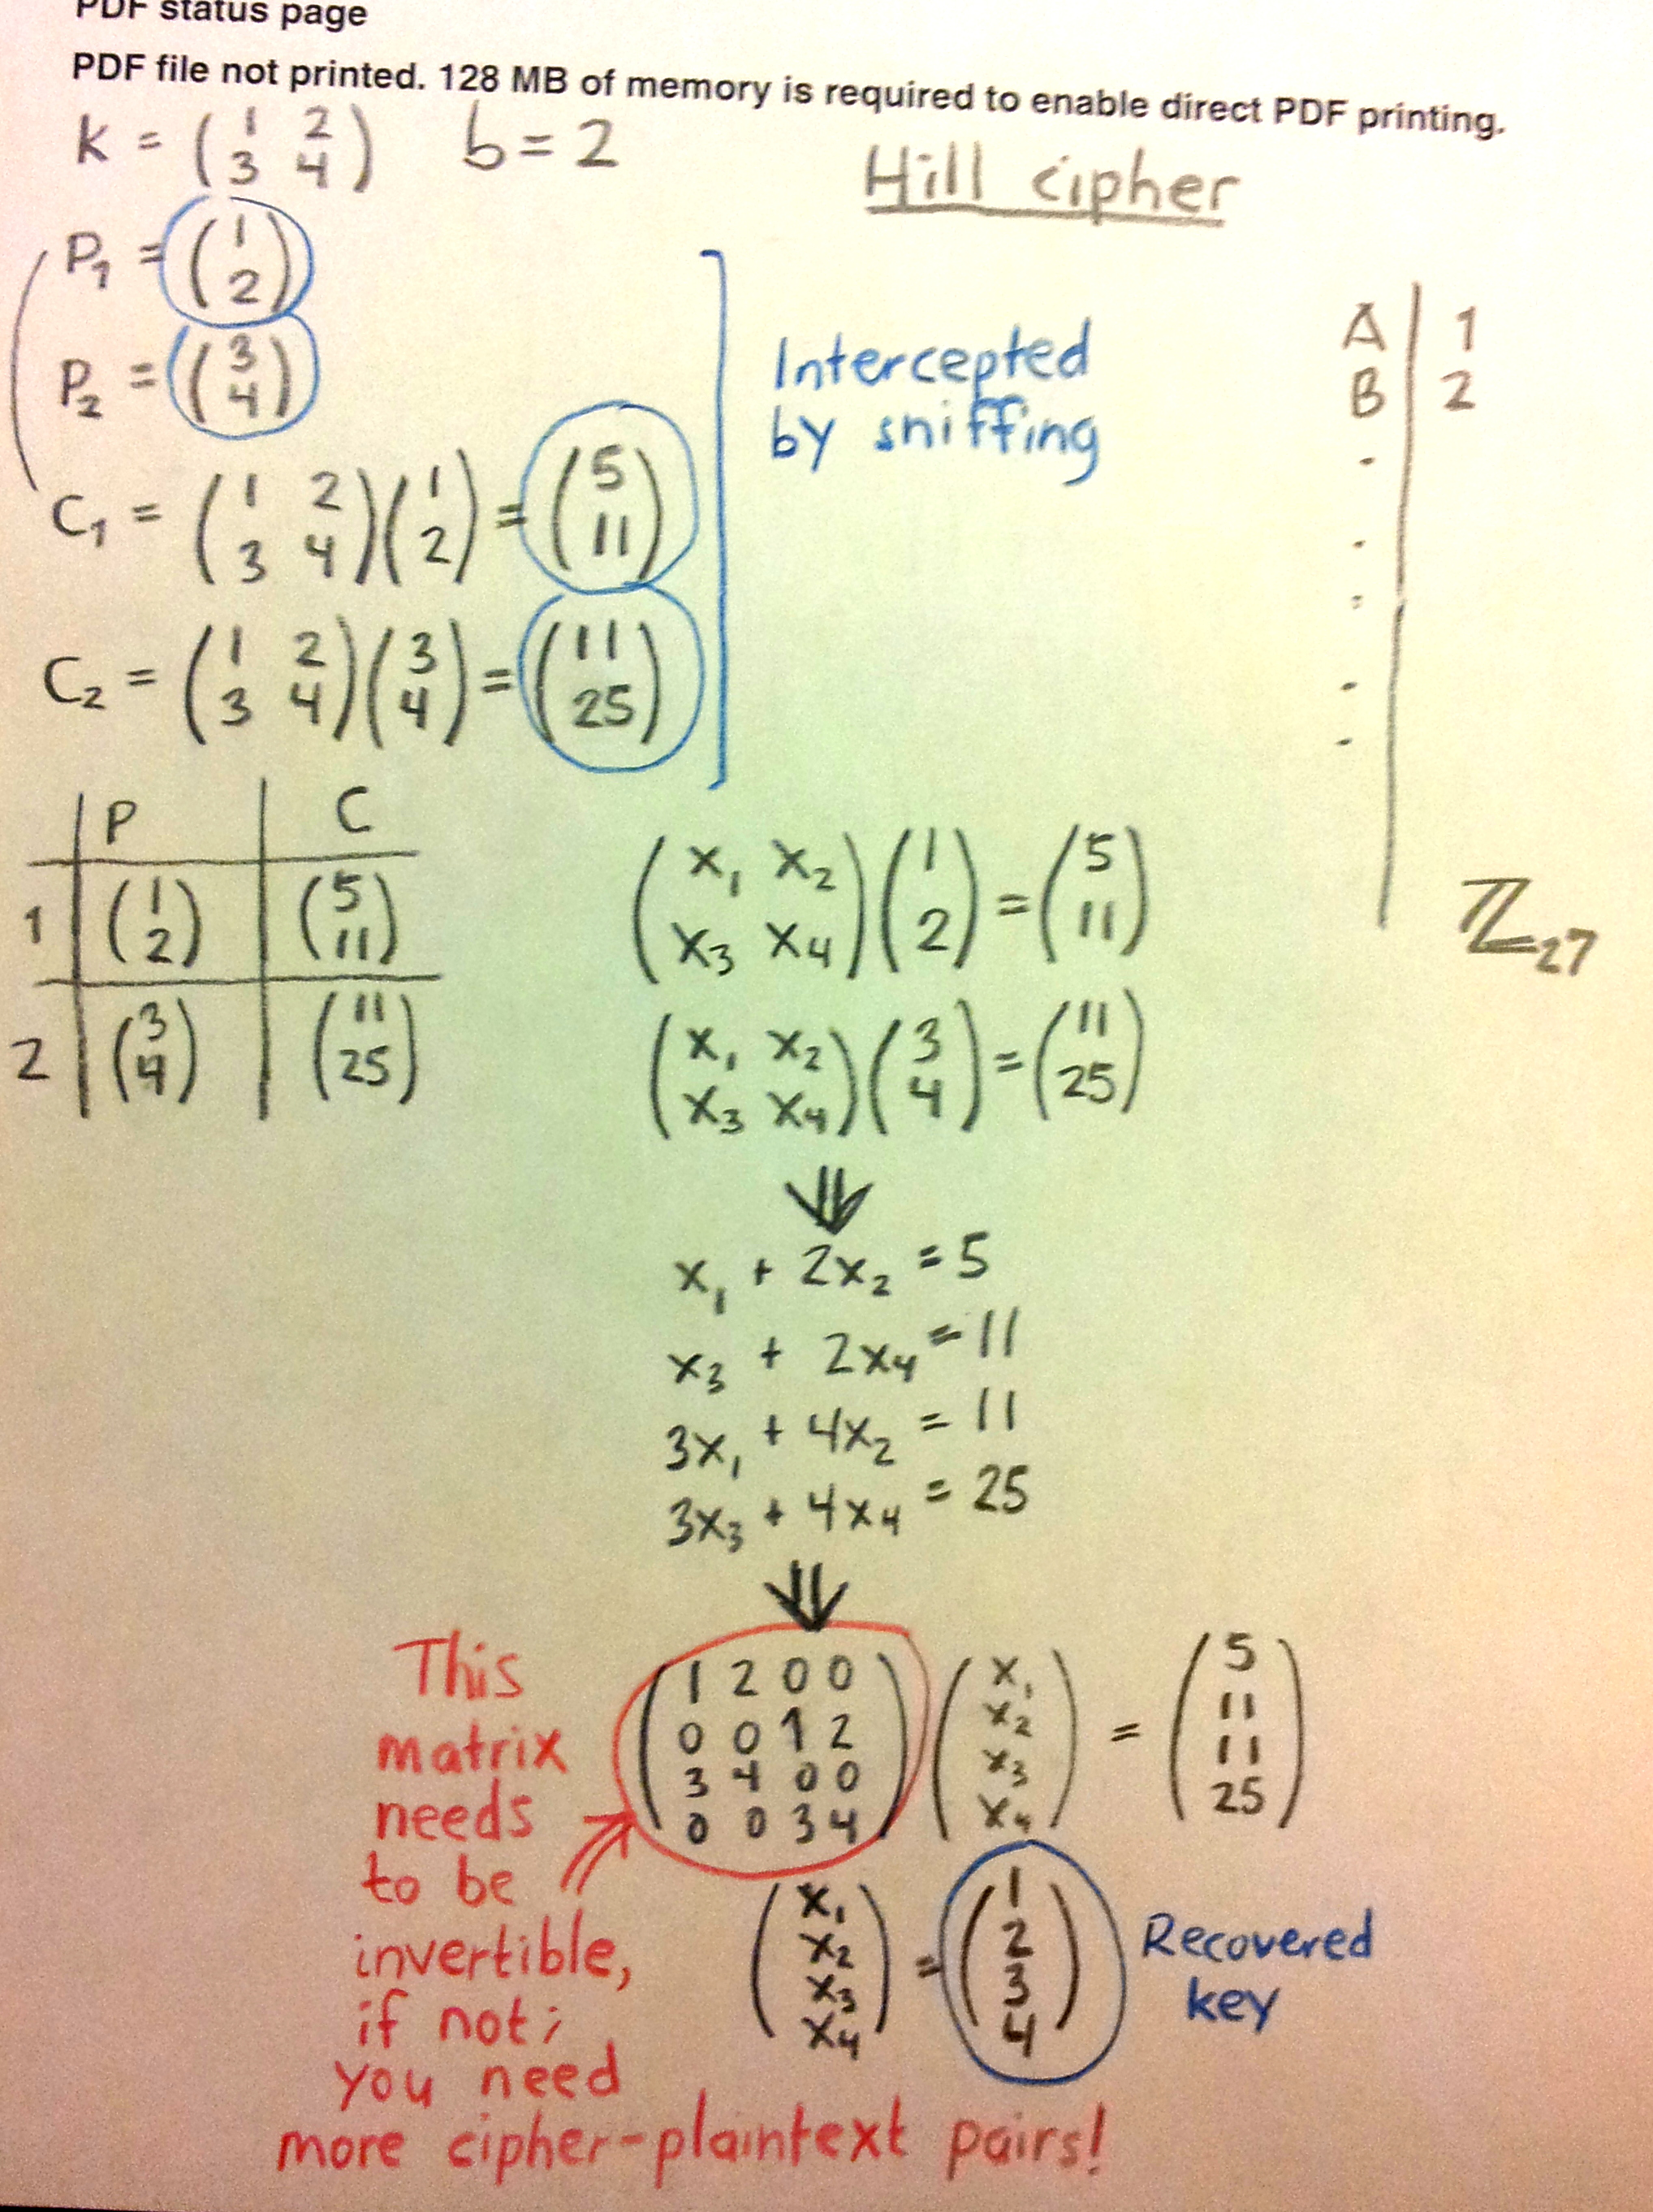
\includegraphics[width=120mm]{hill.jpg}
\caption{Breaking the Hill cipher with pen and paper.}
\end{figure}
\end{problem}

Breaking the cipher involves inversion of a matrix and matrix multiplication. The worst time complexity for these operations are $O(b^3)$. 
\begin{problem} % Problem 6 - School ciphers
  (5T) I would assume they would come up with a simple cipher like the Ceasar cipher where
  you substitute letters with other letters. 
  
  Unless you make your cipher a little bit more complicated you usually end up with a small keyspace. For example, in the Shift Cipher, the key is the number of steps you shift each letter, so the keyspace is usually restricted to the number of letters in the alphabet.  If it was a Swedish school, I would assume that they encrypt messages written in Swedish. In that case you can make a program which tests all possible keys until something like Swedish pops up. The program can use a wordlist to determine if the ciphertext was decrypted with the correct key. 
  
  If a brute-force attack is infeasible, I would try to make some kind of frequency analysis. My program would count the number of occurrences for each letter and compare it with known statistics. For example, in Swedish, the most common letters are $e$ and $a$, so one might assume that the most common letters in the ciphertext correspond to any of these two letters. My program would try to replace letters from the ciphertext in this way, until I retrieve some Swedish words. The "gaps" could probably be decrypted manually. I would also look at combinations with two- or maybe three letters (bi- and trigrams) and subsititute blocks of text like described above.
\end{problem}

\begin{problem} % Problem 7 - Adversaries
  \begin{subproblem}
    (1T) First off, an adversary is a malicious opponent trying to break e.g the cryptographic scheme used. Each crypto scheme has a security parameter, for example in RSA, it's the size of the prime numbers that need to be factored. The difference between uniform and non-uniform adversaries lies in whether their behavior is computable when the value of the security parameter is changed. As far as I understand, a uniform adversary is like a deterministic turing machine. It always runs the same program to break the crypytographic scheme. Although the behavior might change over time, it is always defined by the program being executed and thus computable. A non-uniform adversary is like a non-deterministic turing machine that can run many different programs depending on the value of the security parameter. In the nature of the NTM lies the property of always choosing the "best" attack, since this is not known beforehand, its actions are non-computable. A non-uniform adversary is considered a harder opponent than the uniform adversary. 
  \end{subproblem}
  \begin{subproblem}
    (2T) As already mentioned, the non-uniform adversary is more powerful. For security reasons, one should assume a non-uniform adversary. However, in practice I think adversaries are uniform.
  \end{subproblem}
\end{problem}

\begin{problem} % Problem 8 -- Feistel networks 
  \begin{subproblem}
    (1T) See separate paper.
  \end{subproblem}
  \begin{subproblem}
    (2T) If we only apply one round Feistel then $L_{1} = R_{0}$. So the left part of the ciphertext
    is clearly not psuedorandom, because it is exactly equal to the right part of the plaintext.
  \end{subproblem}
  \begin{subproblem}
    (4T) Lets assume that we input two blocks $L_{1} || R$ and $L_{2} || R$ into a Feistel
    network and run two rounds. The output is then $f(R) \oplus L_{1} || f(f(R) \oplus L_{1}) \oplus R$ and $f(R) \oplus L_{2} || f(f(R) \oplus L_{2}) \oplus R$ respectively. If you xor the leftmost $\frac{n}{2}$ bits of the two outputs with each other you get:
    \[ (f(R) \oplus L_{1}) \oplus (f(R) \oplus L_{2}) = f(R) \oplus f(R) \oplus L_{1} \oplus L_{2} = L_{1} \oplus L_{2}
    \]
    Even though we don't know the actual bits $f(R) \oplus L_{i}$ because it is dependent on the key; if we xor it with another ciphertext having the same $\frac{n}{2}$ rightmost bits, the xor differential is no longer dependent on the key, hence it's not psuedorandom. 
  \end{subproblem}
  \begin{subproblem}
    (10T) NOT SOLVED % We leave this place holder here for improved readability.
  \end{subproblem}
\end{problem}

\end{document}